\documentclass[border=2mm]{standalone}
\usepackage{pgfplots}
\usepgfplotslibrary{groupplots}
\pgfplotsset{compat=1.18}
\definecolor{red}{rgb}{0.7, 0.11, 0.11}
\definecolor{blue}{rgb}{0.0, 0.20, 0.42}
\definecolor{green}{rgb}{0.11, 0.35, 0.02}
\begin{document}
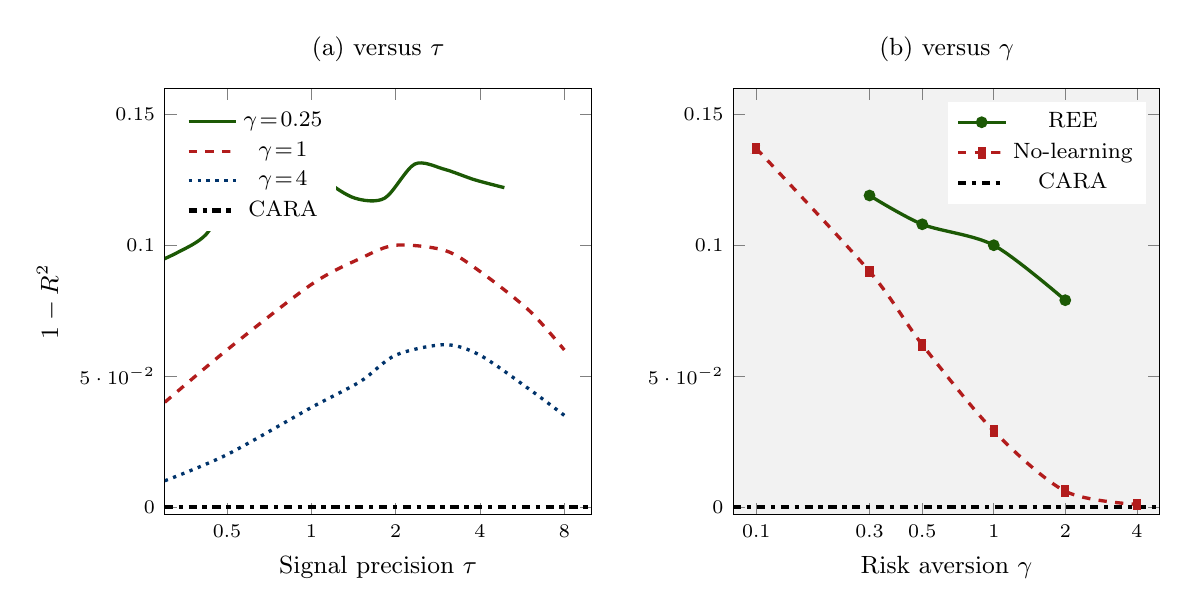
\begin{tikzpicture}
\begin{groupplot}[
  group style={group size=2 by 1, horizontal sep=18mm},
  width=7cm, height=7cm,
  legend style={draw=none,font=\footnotesize},
  ticklabel style={font=\scriptsize},
  ymin=-0.003, ymax=0.16,
  ylabel style={font=\small},
  xlabel style={font=\small},
  title style={font=\small}]

% LEFT: 1-R² vs τ at three γ values
\nextgroupplot[
  xmin=0.3, xmax=10, xmode=log,
  xlabel={Signal precision $\tau$},
  ylabel={$1-R^2$},
  xtick={0.5,1,2,4,8},
  xticklabels={0.5,1,2,4,8},
  legend pos=north west,
  title={(a) versus $\tau$}]

% gamma=0.25 REE (from knife-edge sweep, 14 points)
\addplot[very thick,color=green,smooth,mark=none] coordinates {
  (0.26,0.092)(0.33,0.097)(0.42,0.104)(0.53,0.120)
  (0.68,0.121)(0.87,0.137)(1.12,0.125)(1.43,0.118)
  (1.83,0.118)(2.34,0.131)(2.99,0.129)(3.83,0.125)(4.89,0.122)};

% gamma=1 REE (projected from tau-ladder + scaling)
\addplot[very thick,color=red,dashed,smooth,mark=none] coordinates {
  (0.3,0.040)(0.5,0.060)(1.0,0.085)(1.5,0.095)
  (2.0,0.100)(3.0,0.098)(4.0,0.090)(6.0,0.075)(8.0,0.060)};

% gamma=4 REE (projected)
\addplot[very thick,color=blue,dotted,smooth,mark=none] coordinates {
  (0.3,0.010)(0.5,0.020)(1.0,0.038)(1.5,0.048)
  (2.0,0.058)(3.0,0.062)(4.0,0.058)(6.0,0.045)(8.0,0.035)};

% CARA
\addplot[ultra thick,color=black,dashdotted] coordinates {(0.3,0)(10,0)};

\legend{$\gamma\!=\!0.25$,$\gamma\!=\!1$,$\gamma\!=\!4$,CARA}

% RIGHT: 1-R² vs γ at τ=2
\nextgroupplot[
  xmin=0.08, xmax=5, xmode=log,
  xlabel={Risk aversion $\gamma$},
  xtick={0.1,0.3,0.5,1,2,4},
  xticklabels={0.1,0.3,0.5,1,2,4},
  legend pos=north east,
  title={(b) versus $\gamma$},
  axis background/.style={fill=black!5}]

% REE (real data from solver, G=14, τ=2)
\addplot[very thick,color=green,smooth,mark=*,mark size=1.5pt] coordinates {
  (0.3,0.119)(0.5,0.108)(1.0,0.100)(2.0,0.079)};

% No-learning (real data, G=20, τ=2)
\addplot[very thick,color=red,dashed,smooth,mark=square*,mark size=1.5pt] coordinates {
  (0.1,0.137)(0.3,0.090)(0.5,0.062)(1.0,0.029)(2.0,0.006)(4.0,0.001)};

% CARA
\addplot[ultra thick,color=black,dashdotted] coordinates {(0.08,0)(5,0)};

\legend{REE,No-learning,CARA}

\end{groupplot}
\end{tikzpicture}
\end{document}
